\section{Results and Discussion} \label{sec:results}

\subsection{Genealogical Inference}

\begin{sidewaysfigure}

  \begin{subfigure}{.33\linewidth}
    \centering
    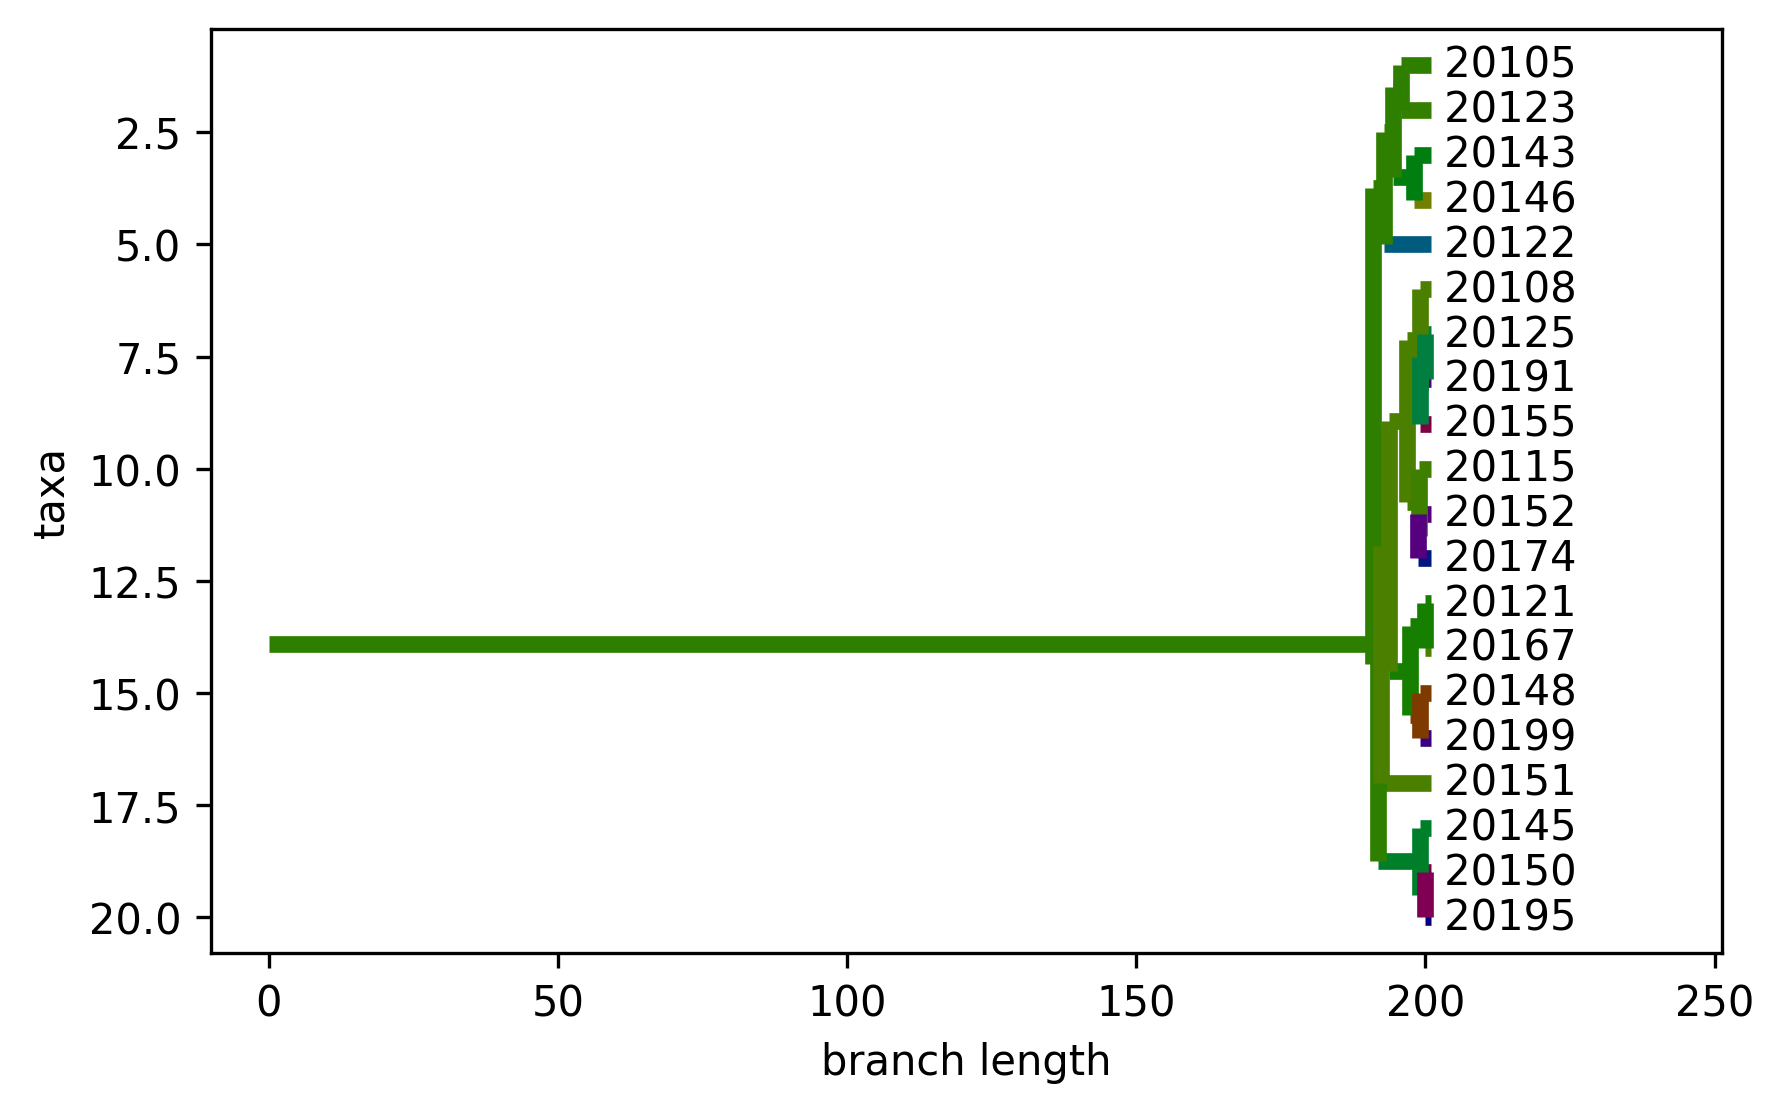
\includegraphics[width=1.05\linewidth]{notebooks/notebooks/teeplots/max_leaves=20+notebook=species-inference+replicate=0+treatment=bag+type=distilled-reference+viz=draw-biopython-tree+ext=}
    \caption{Subcaption 1}
    \label{fig:species-example-replicates:bag-reference}
  \end{subfigure}
  \begin{subfigure}{.33\linewidth}
    \centering
    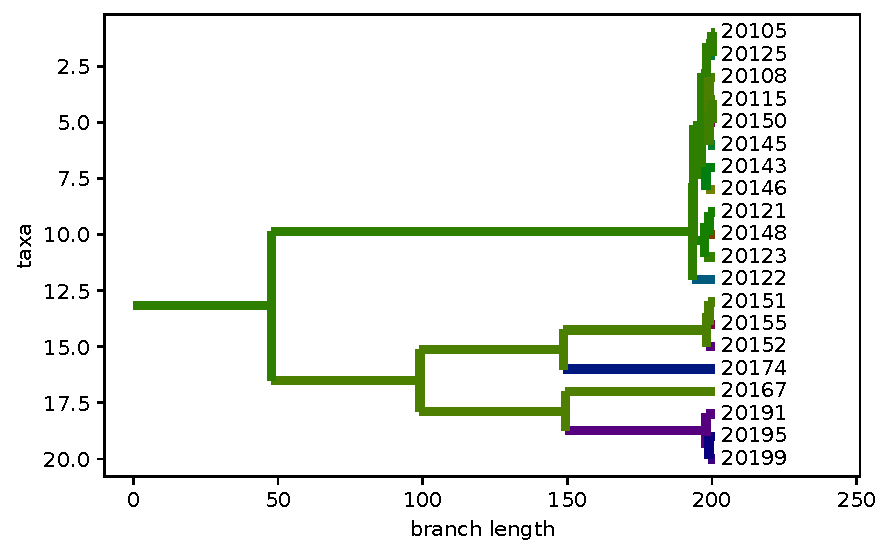
\includegraphics[width=1.05\linewidth]{notebooks/notebooks/teeplots/max_leaves=20+notebook=species-inference+replicate=0+treatment=allopatry+type=distilled-reference+viz=draw-biopython-tree+ext=}
    \caption{Allopatry reference}
    \label{fig:species-example-replicates:allopatry-reference}
  \end{subfigure}
  \begin{subfigure}{.33\linewidth}
    \centering
    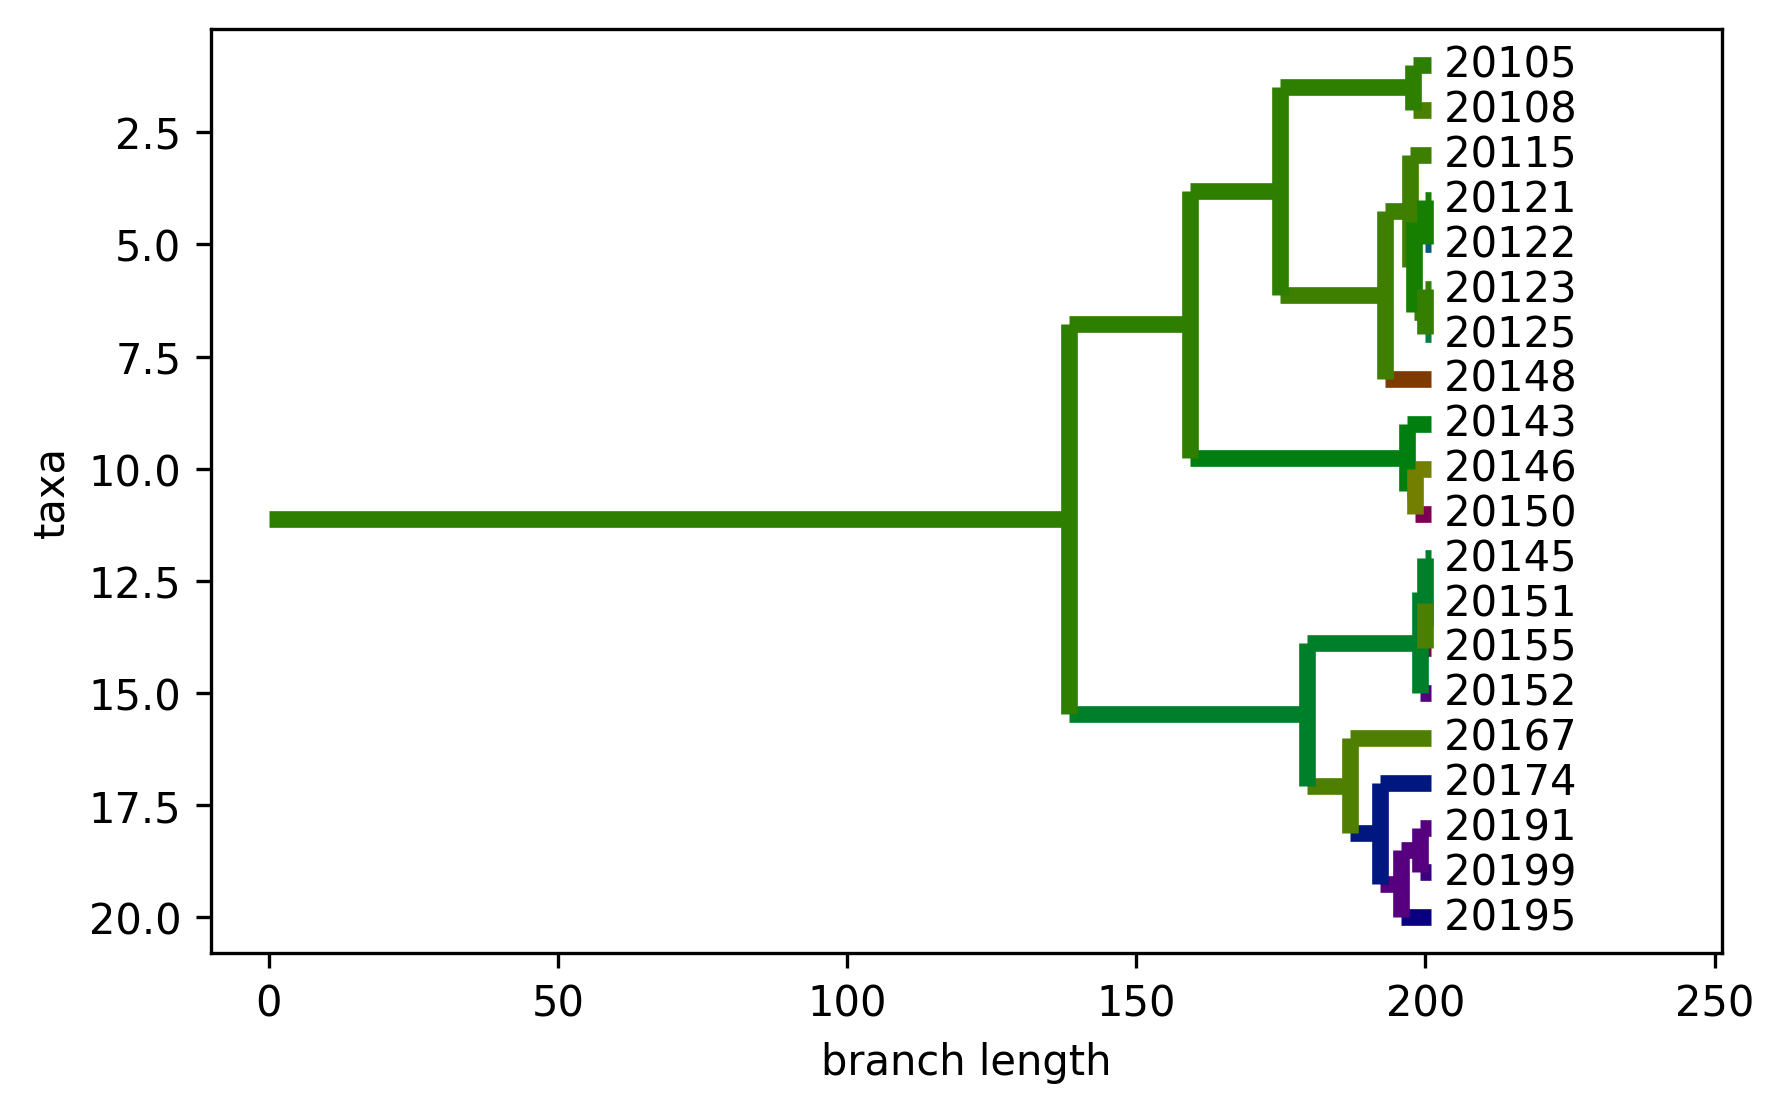
\includegraphics[width=1.05\linewidth]{notebooks/notebooks/teeplots/max_leaves=20+notebook=species-inference+replicate=0+treatment=ring+type=distilled-reference+viz=draw-biopython-tree+ext=}
    \caption{Ring reference}
    \label{fig:species-example-replicates:ring-reference}
  \end{subfigure}

  \begin{subfigure}{.33\linewidth}
    \centering
    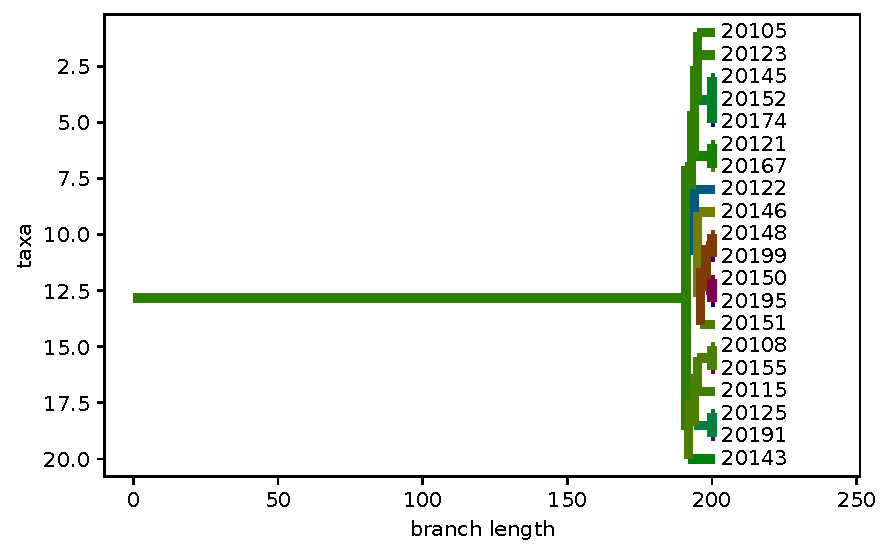
\includegraphics[width=1.05\linewidth]{notebooks/notebooks/teeplots/max_leaves=20+notebook=species-inference+replicate=0+treatment=bag+type=reconstruction+viz=draw-biopython-tree+ext=}
    \caption{Bag reconstruction}
    \label{fig:species-example-replicates:bag-reconstruction}
  \end{subfigure}
  \begin{subfigure}{.33\linewidth}
    \centering
    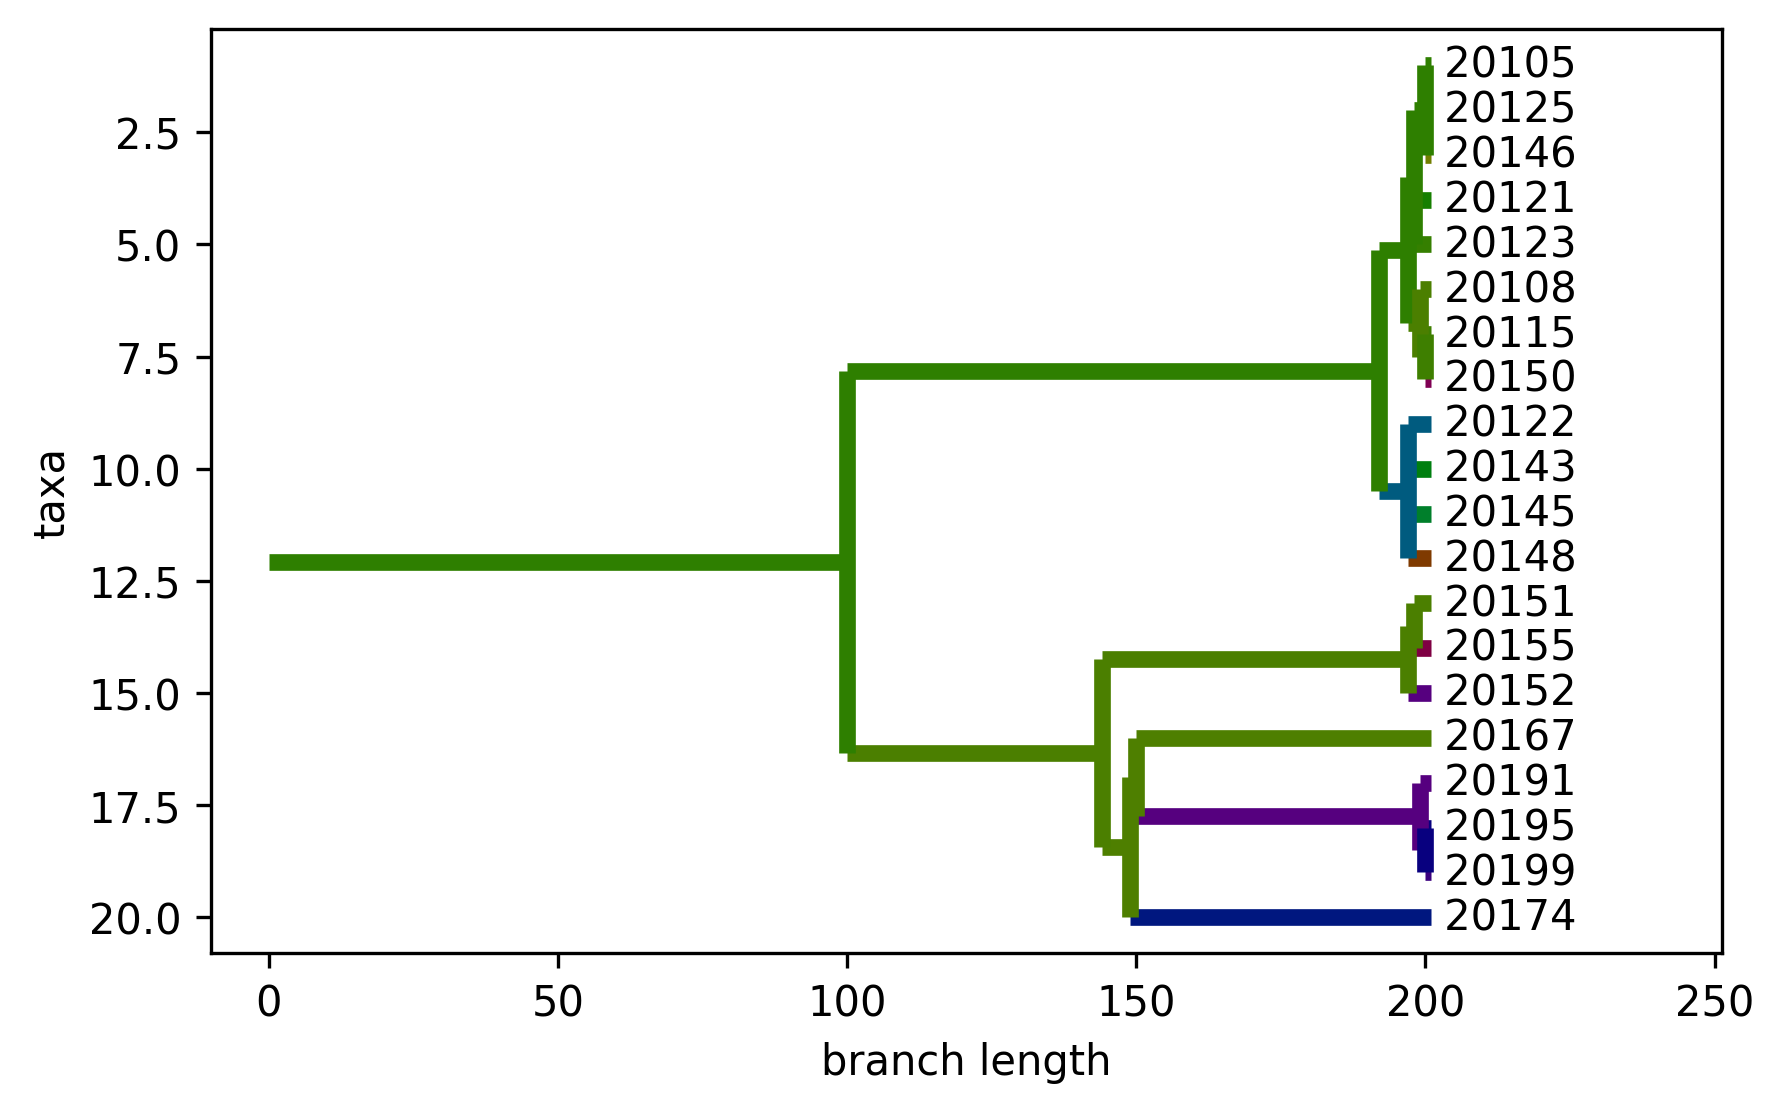
\includegraphics[width=1.05\linewidth]{notebooks/notebooks/teeplots/max_leaves=20+notebook=species-inference+replicate=0+treatment=allopatry+type=reconstruction+viz=draw-biopython-tree+ext=}
    \caption{Allopatry reconstruction}
    \label{fig:species-example-replicates:allopatry-reconstruction}
  \end{subfigure}
  \begin{subfigure}{.33\linewidth}
    \centering
    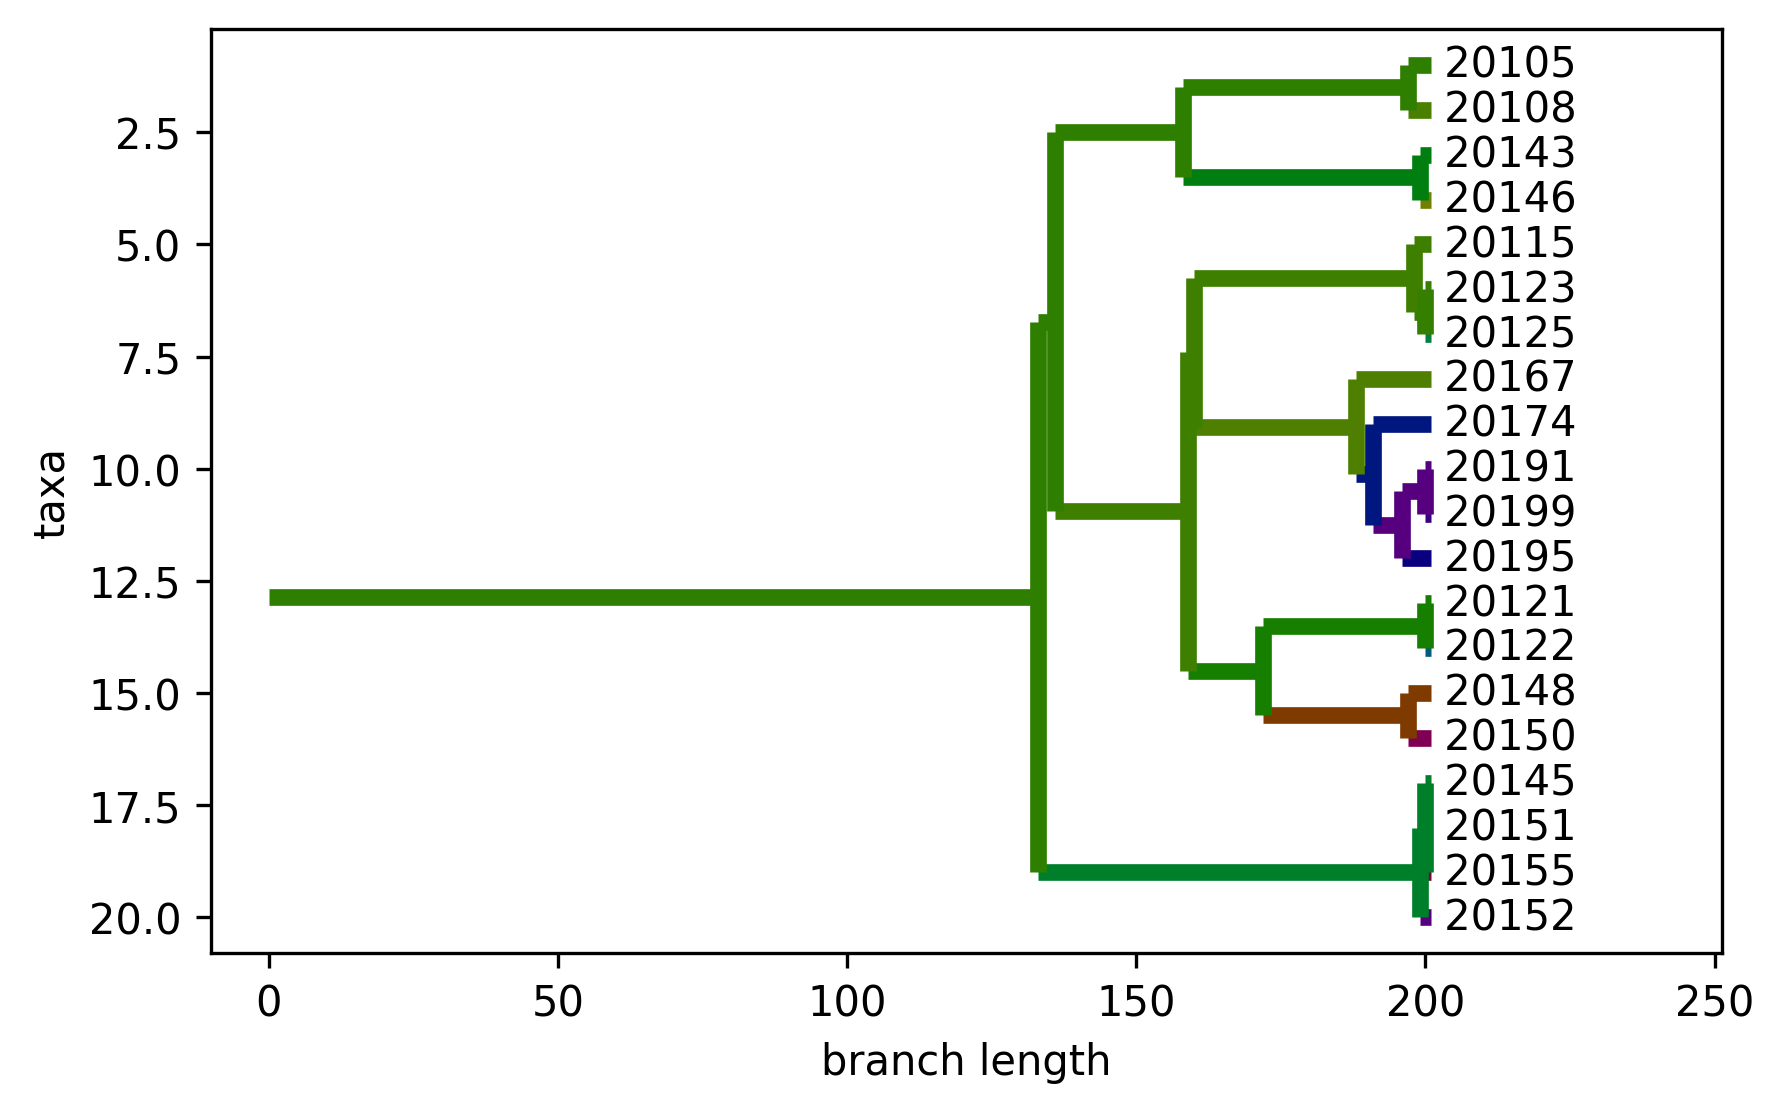
\includegraphics[width=1.05\linewidth]{notebooks/notebooks/teeplots/max_leaves=20+notebook=species-inference+replicate=0+treatment=ring+type=reconstruction+viz=draw-biopython-tree+ext=}
    \caption{Ring reconstruction}
    \label{fig:species-example-replicates:ring-reconstruction}
  \end{subfigure}

  \caption{Caption for the whole figure}
  \label{fig:species-example-replicates}

\end{sidewaysfigure}
%
% notebooks/notebooks/teeplots/max_leaves=20+notebook=species-inference+replicate=0+treatment=allopatry+type=distilled-reference+viz=draw-biopython-tree+ext=.pdf
%
% notebooks/notebooks/teeplots/max_leaves=20+notebook=species-inference+replicate=0+treatment=allopatry+type=reconstruction+viz=draw-biopython-tree+ext=.pdf
%
% notebooks/notebooks/teeplots/max_leaves=20+notebook=species-inference+replicate=0+treatment=bag+type=distilled-reference+viz=draw-biopython-tree+ext=.pdf
%
% notebooks/notebooks/teeplots/max_leaves=20+notebook=species-inference+replicate=0+treatment=bag+type=reconstruction+viz=draw-biopython-tree+ext=.pdf
%
% notebooks/notebooks/teeplots/max_leaves=20+notebook=species-inference+replicate=0+treatment=ring+type=distilled-reference+viz=draw-biopython-tree+ext=.pdf
%
% notebooks/notebooks/teeplots/max_leaves=20+notebook=species-inference+replicate=0+treatment=ring+type=reconstruction+viz=draw-biopython-tree+ext=.pdf


Figure \ref{fig:species-example-replicates} compares phylogenetic trees reconstructed from to corresponding references extracted from perfectly-tracked sexual pedigrees.
For treatments with meaningful phylogentic structure --- the ``allopatry'' and ``ring'' treatments --- phylogenetic reconstruction from species-level annotation largely succeeded in recovering membership in structured subpopulations and the historical relationships between subpopulations.
In fact, for the ``allopatry'' treatment, inner node time points appear to more closely track the true generational time frames of speciation events (at generation 100 and 150) than the UPGMA-based pedigree distillation.
Adherence to the reference structure is somewhat weaker in the ring treatment than the allopatry treatment, perhaps due to ill-definedness of nontransitive phylogenetic distances expected due to genetic relatedness closing around the ring in both directions.
Reconstruction/reference comparisons for other replicates will be provided in supplemental material.

\begin{SCfigure}[3]
  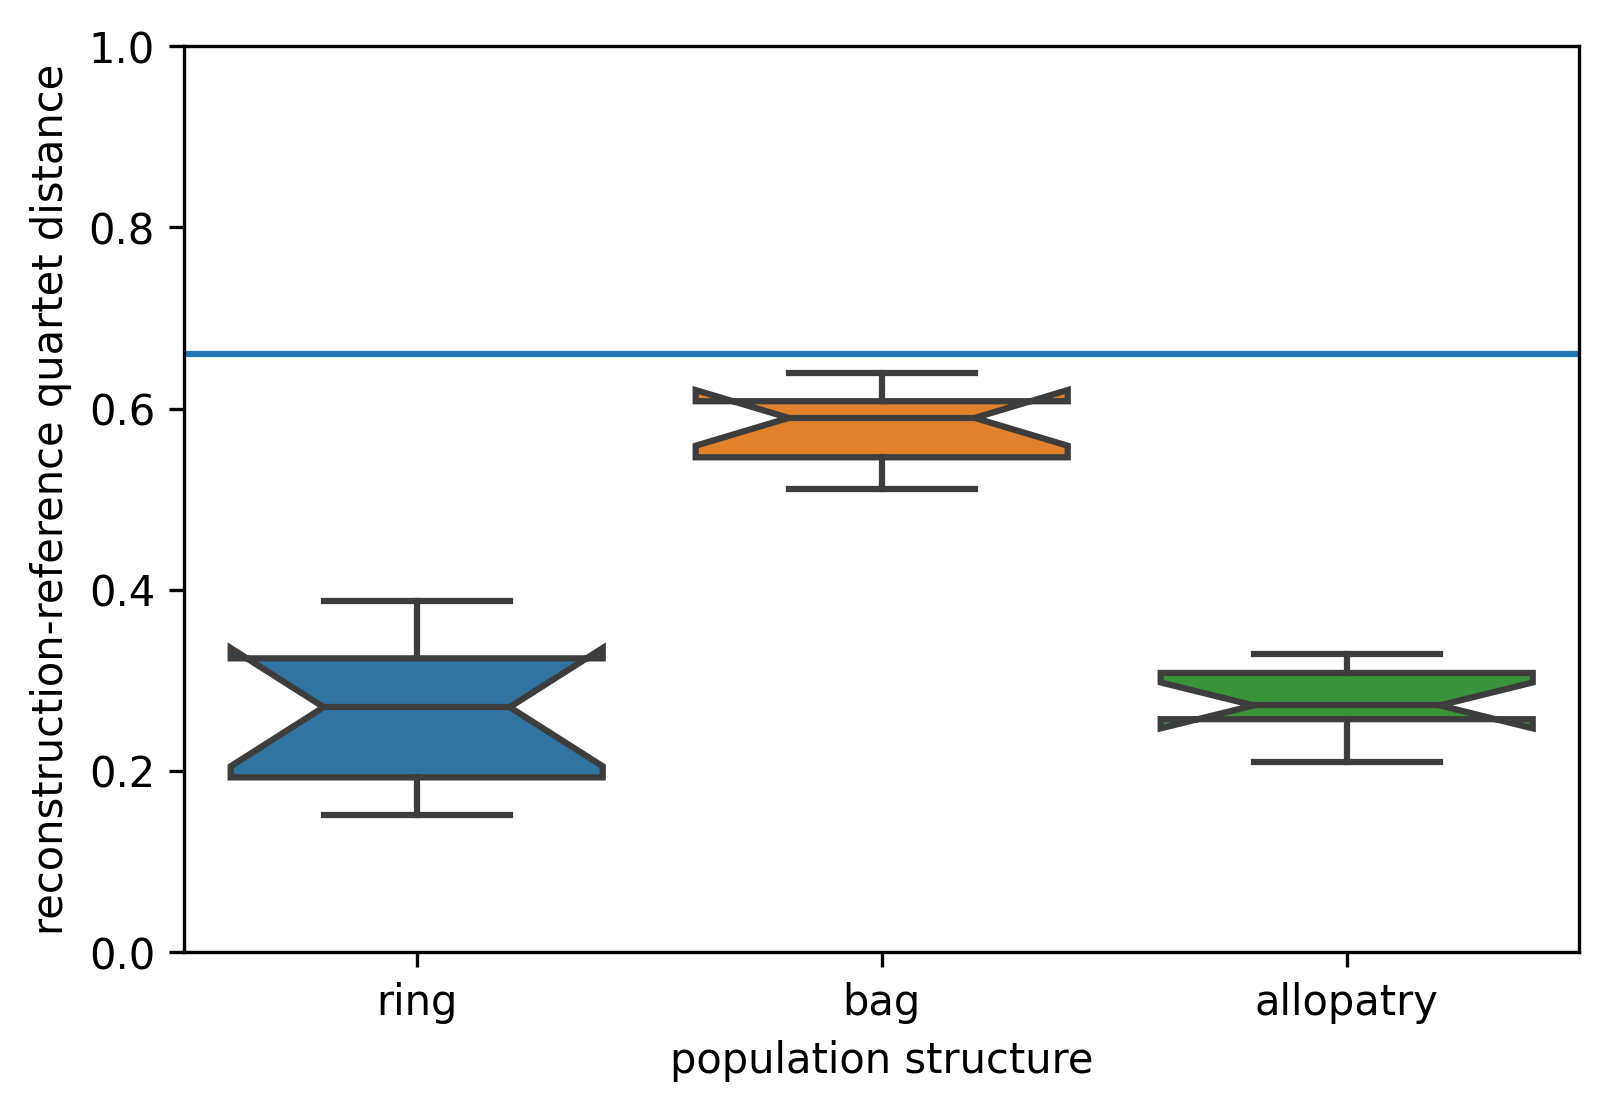
\includegraphics[width=0.5\textwidth]{notebooks/notebooks/teeplots/viz=boxplot-quartet+x=treatment+y=quartet-distance+ext=}
  \caption{
    Normalized quartet distances between reconstructed phylogenies and references distilled from tracked pedigree.
    Lower indicates less reconstruction error.
    Notches give bootstrapped 95\% CI.
    Horizontal blue line indicates expected quartet distance between random trees.
    Some reconstruction error is expected, especially in control treatment, due to resolution of effectively arbitrary phylogenetic structure among well-mixed population components.
  }
  \label{fig:species-reconstruction-error}
\end{SCfigure}


Figure \ref{fig:species-reconstruction-error} shows distributions of reconstruction error for each treatment.

Across all three treatments, all ten replicate reconstructions exhibited quartet distance from reference was strictly less than 0.66, the expected quartet distance between random trees \citep{smith2020information}.
This provides strong evidence that some successful phylogenetic inference occurred in all three cases (exact binomial test, $p < 0.01$).

However, as expected, reconstruction quality on the bag population structure was marginal due to the lack of meaningful phylogenetic information to reconstruct.
Performance on the ring and allopatry treatments was stronger, achieving quartet distances between reconstruction and reference of around 0.3 in the typical case.
Inclusion of nebulous phylogenetic structure within the reference phylogeny (i.e., within well-mixed subpopulations in both ) seems likely to significantly contribute to reconstruction error, obscuring the true magnitude of meaningful reconstruction error due to limitations of the instrumentation-based approach.
More sophisticated pedigree-to-phylogeny conversion that collapses closely-related subpopulations to single nodes may prove more descriptive.

\subsection{Effective Population Size Inference}

\begin{figure}
  \centering
  \begin{minipage}{\textwidth} % adjust the width as needed

    \begin{minipage}{0.5\textwidth}
      \centering
      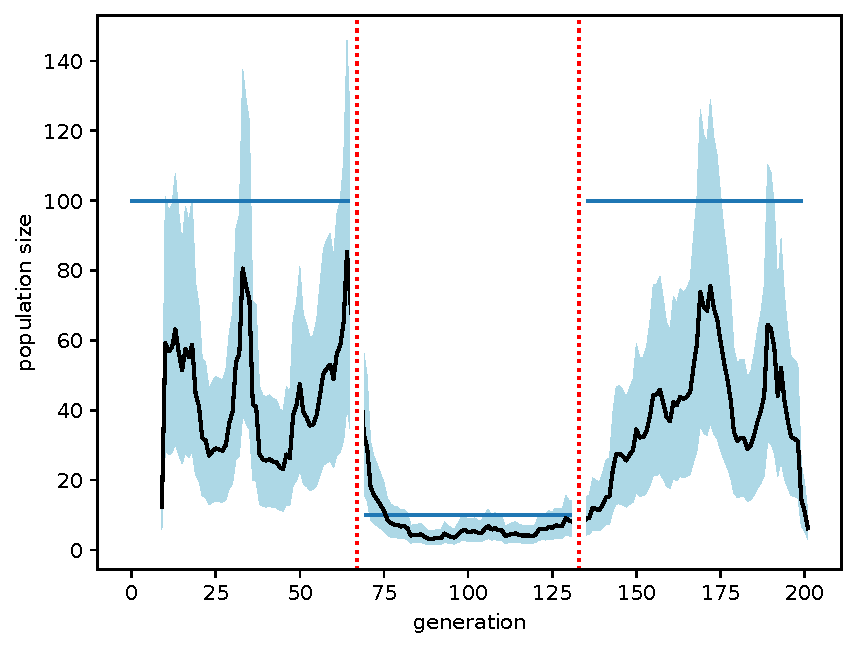
\includegraphics[height=0.23\textheight]{notebooks/notebooks/teeplots/notebook=ne-inference+replicate=0+treatment=bottleneck+viz=plot-running-estimation+x=rank+y=population-size+ext=}
      \subcaption{Bottleneck treatment}
      \label{fig:ne-example-replicates:bottleneck}
    \end{minipage}%
    \begin{minipage}{0.5\textwidth}
      \centering
      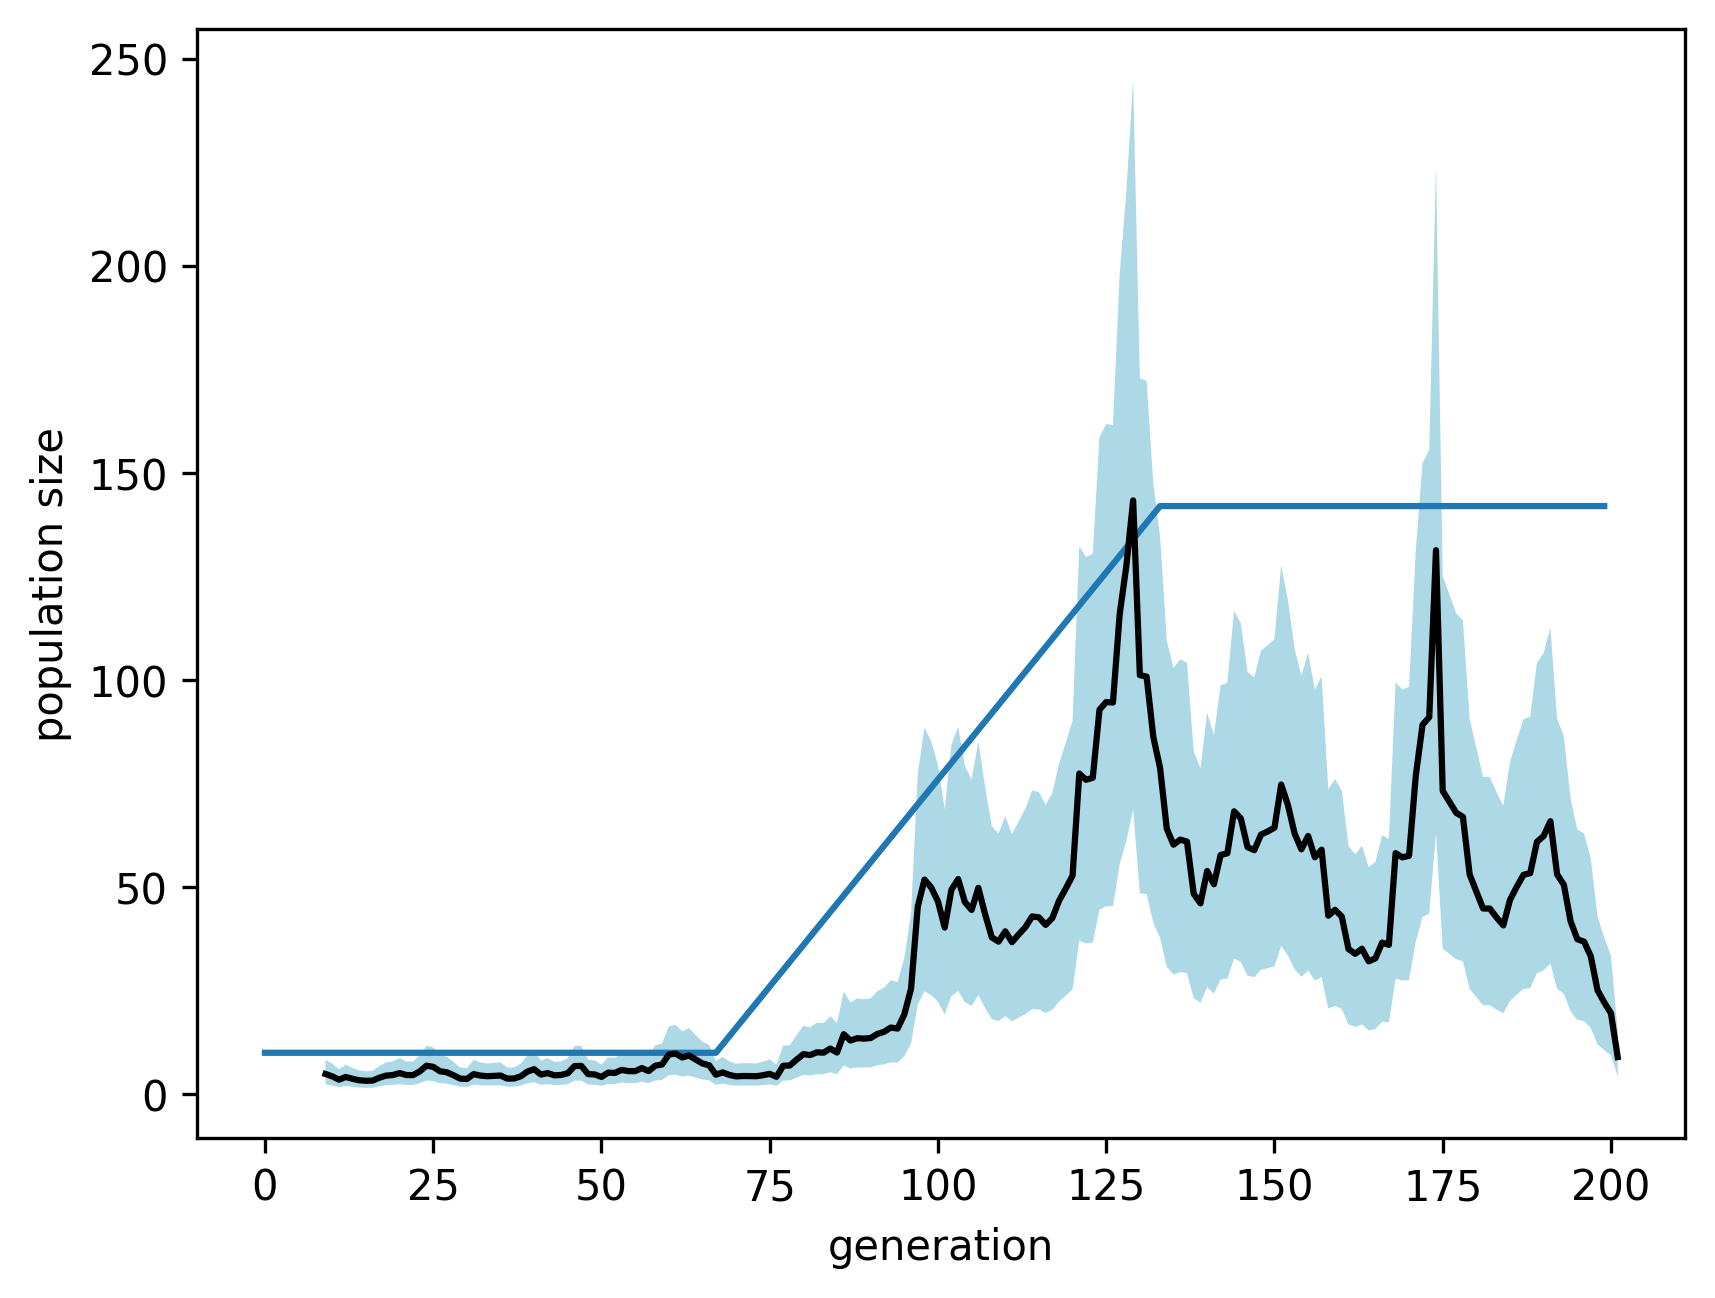
\includegraphics[height=0.23\textheight]{notebooks/notebooks/teeplots/notebook=ne-inference+replicate=0+treatment=range-expansion+viz=plot-running-estimation+x=rank+y=population-size+ext=}
      \subcaption{Range expansion treatment}
      \label{fig:ne-example-replicates:range_expansion}
    \end{minipage}

    \begin{minipage}{0.5\textwidth}
      \centering
      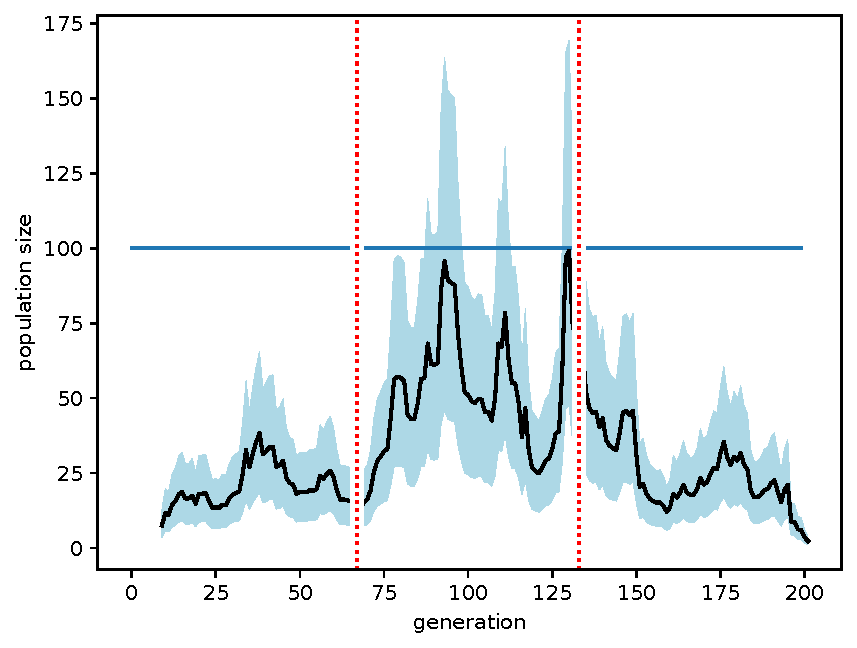
\includegraphics[height=0.23\textheight]{notebooks/notebooks/teeplots/notebook=ne-inference+replicate=0+treatment=selection-pressure+viz=plot-running-estimation+x=rank+y=population-size+ext=}
      \subcaption{Selection pressure treatment}
      \label{fig:ne-example-replicates:selection_pressure}
    \end{minipage}%
    \begin{minipage}{0.5\textwidth}
      \centering
      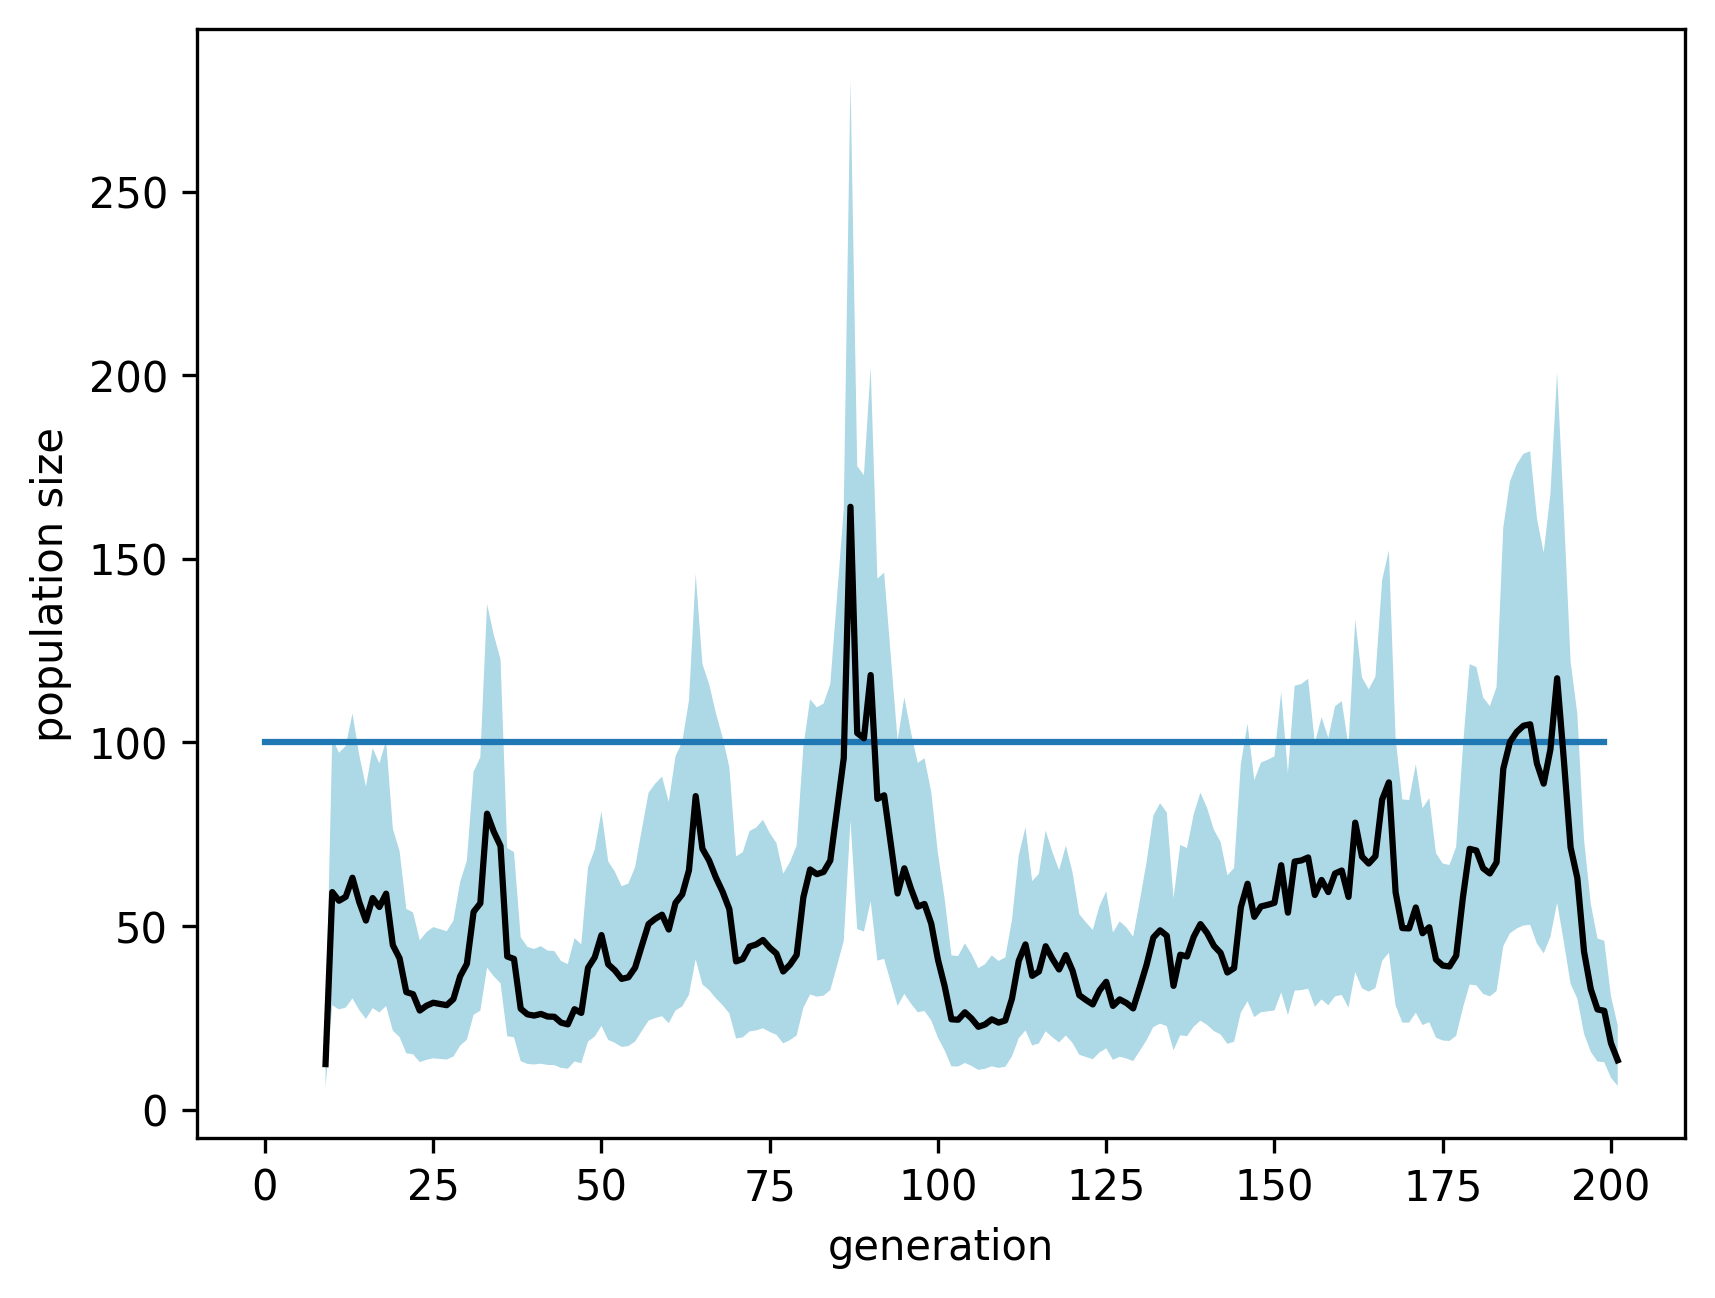
\includegraphics[height=0.23\textheight]{notebooks/notebooks/teeplots/notebook=ne-inference+replicate=0+treatment=control+viz=plot-running-estimation+x=rank+y=population-size+ext=}
      \subcaption{Control treatment}
      \label{fig:ne-example-replicates:control}
    \end{minipage}

  \end{minipage}
  \hfill % Creates horizontal space. Can also use \hspace{<len>}
  \begin{minipage}{\textwidth} % adjust the width as needed
    \vspace{2ex}
    \caption{Ten-sample running MLE estmate of effective population size of example replicates from  each treatment.
    Shaded region corresponds to 95\% MLE confidence interval.
    Horizontal blue lines indicate true population size.
    Dashed vertical lines indicate treatment discontinuities.
    See Section \ref{sec:population-size-inference-experiments} for population size and selection pressure manipulations performed for each treatment.
    Note that disparity between estimated effective population size and true population size is expected due to demographic factors depressing effective population size.
    }
    \label{fig:ne-example-replicates}
  \end{minipage}

\end{figure}


% notebooks/notebooks/teeplots/notebook=ne-inference+replicate=0+treatment=bottleneck+viz=plot-running-estimation+x=rank+y=population-size+ext=.pdf
%
% notebooks/notebooks/teeplots/notebook=ne-inference+replicate=0+treatment=control+viz=plot-running-estimation+x=rank+y=population-size+ext=.pdf
%
% notebooks/notebooks/teeplots/notebook=ne-inference+replicate=0+treatment=range-expansion+viz=plot-running-estimation+x=rank+y=population-size+ext=.pdf
%
% notebooks/notebooks/teeplots/notebook=ne-inference+replicate=0+treatment=selection-pressure+viz=plot-running-estimation+x=rank+y=population-size+ext=.pdf


Figure \ref{fig:ne-example-replicates} compares 10-sample running estimates of population size among one replicate from each surveyed treatment (Section \ref{sec:population-size-inference-experiments}).
Estimate trajectories from other replicates will be made available in supplemental material

All effective population estimates generally appear to respond to underlying demographic changes as expected, although the response to selection pressure relaxation appears somewhat weaker than responses to changes in population size, and orders-of-magnitude-spanning noise appears across all treatments.

\begin{SCfigure}
  \centering
  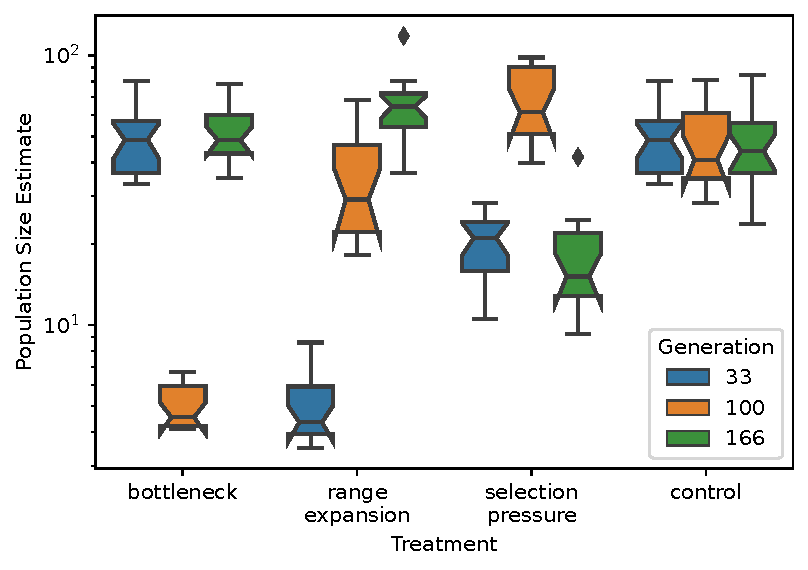
\includegraphics[width=0.6\textwidth]{notebooks/notebooks/teeplots/hue=generation+viz=boxplot-popsize+x=treatment+y=population-size-estimate+ext=}
  \caption{
  Distributions of ten-sample MLE population size estimates by treatment across three time points.
  See Section \ref{sec:population-size-inference} for population size and selection pressure manipulations performed for each treatment.
  Notches indicate bootstrapped 95\% confidence intervals.}
  \label{fig:ne-estimate-distributions}
\end{SCfigure}

% notebooks/notebooks/teeplots/hue=generation+viz=boxplot-popsize+x=treatment+y=population-size-estimate+ext=.pdf


Figure \ref{fig:ne-estimate-distributions} summarizes the distribution of effective population size estimates across replicates at three time points spread across the beginning, middle, and end of evolutionary runs.
Estimates differ significantly across time points within all non-control treatments, confirming population size estimator sensitivity to underlying changes in population size and selection pressure ($p < 0.05$, non-overlapping confidence intervals).
For the bottleneck and selection pressure treatments, which involve reversion to initial conditions, distributions of the first and last time points are comparable, as expected.

\begin{figure}
  \centering

  \begin{subfigure}{\textwidth}
    \begin{minipage}{0.7\textwidth}
      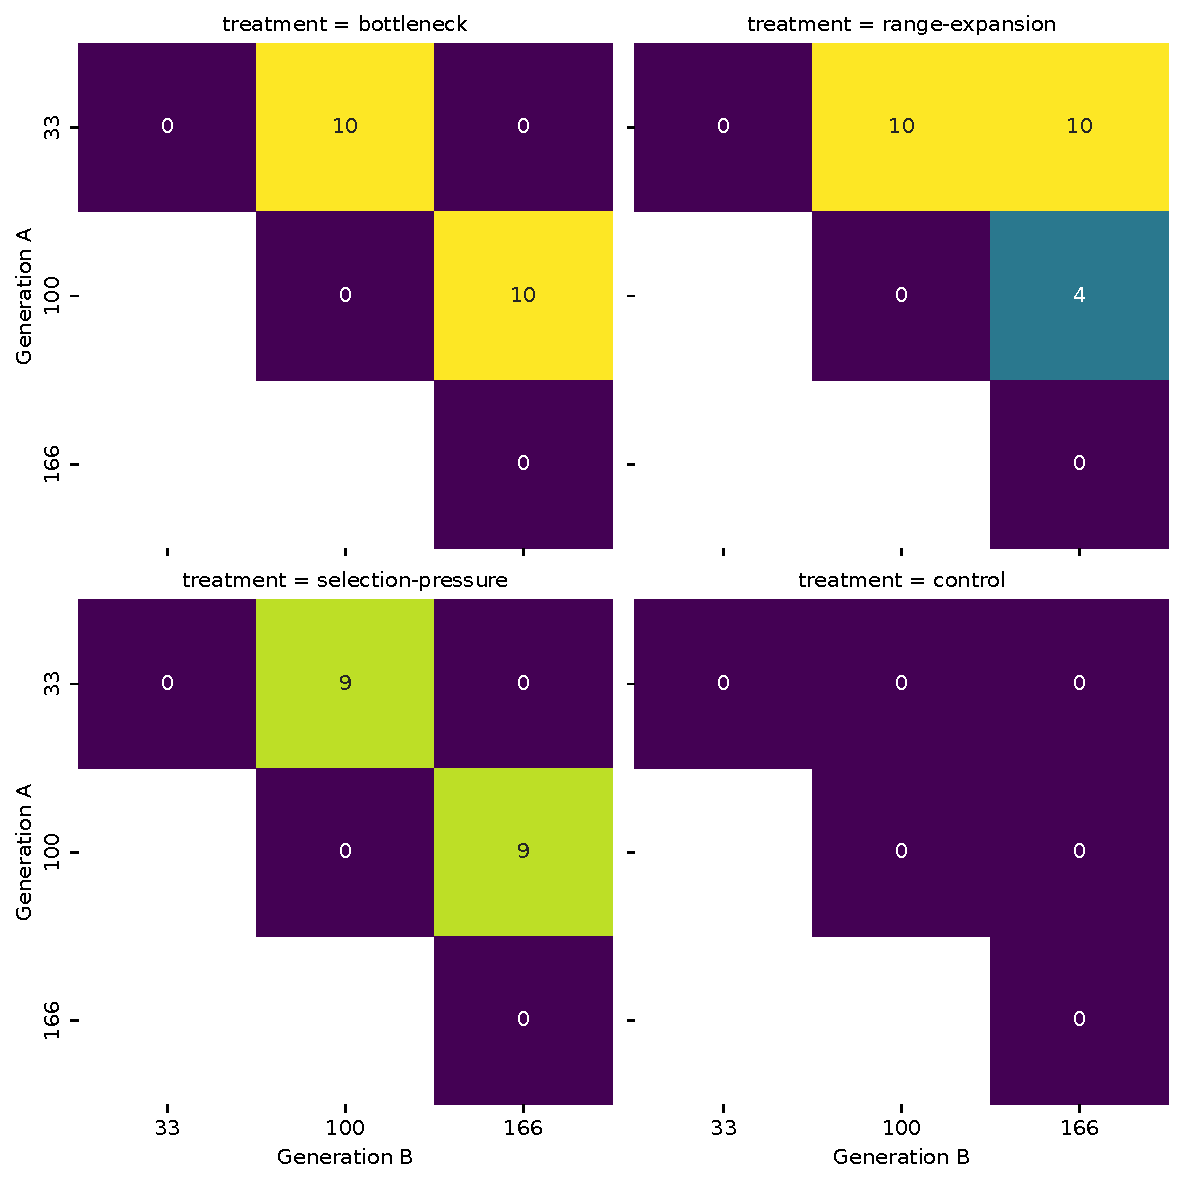
\includegraphics[width=\linewidth]{notebooks/notebooks/teeplots/hue=mann-whitney-significant-at-alpha-0-01+viz=facet-heatmap+x=generation-b+y=generation-a+ext=}
    \end{minipage}%
    \begin{minipage}{0.25\textwidth}
      \caption{Mann-Whitney comparison of 33 annotations at time points surrounding each target generation, with significance threshold $\alpha = 0.01$.}
      \label{fig:ne-detection-matrix:mann-whitney}
    \end{minipage}
  \end{subfigure}

  \vspace{1em} % adjust the vertical spacing between the subfigures

  \begin{subfigure}{\textwidth}
    \begin{minipage}{0.7\textwidth}
      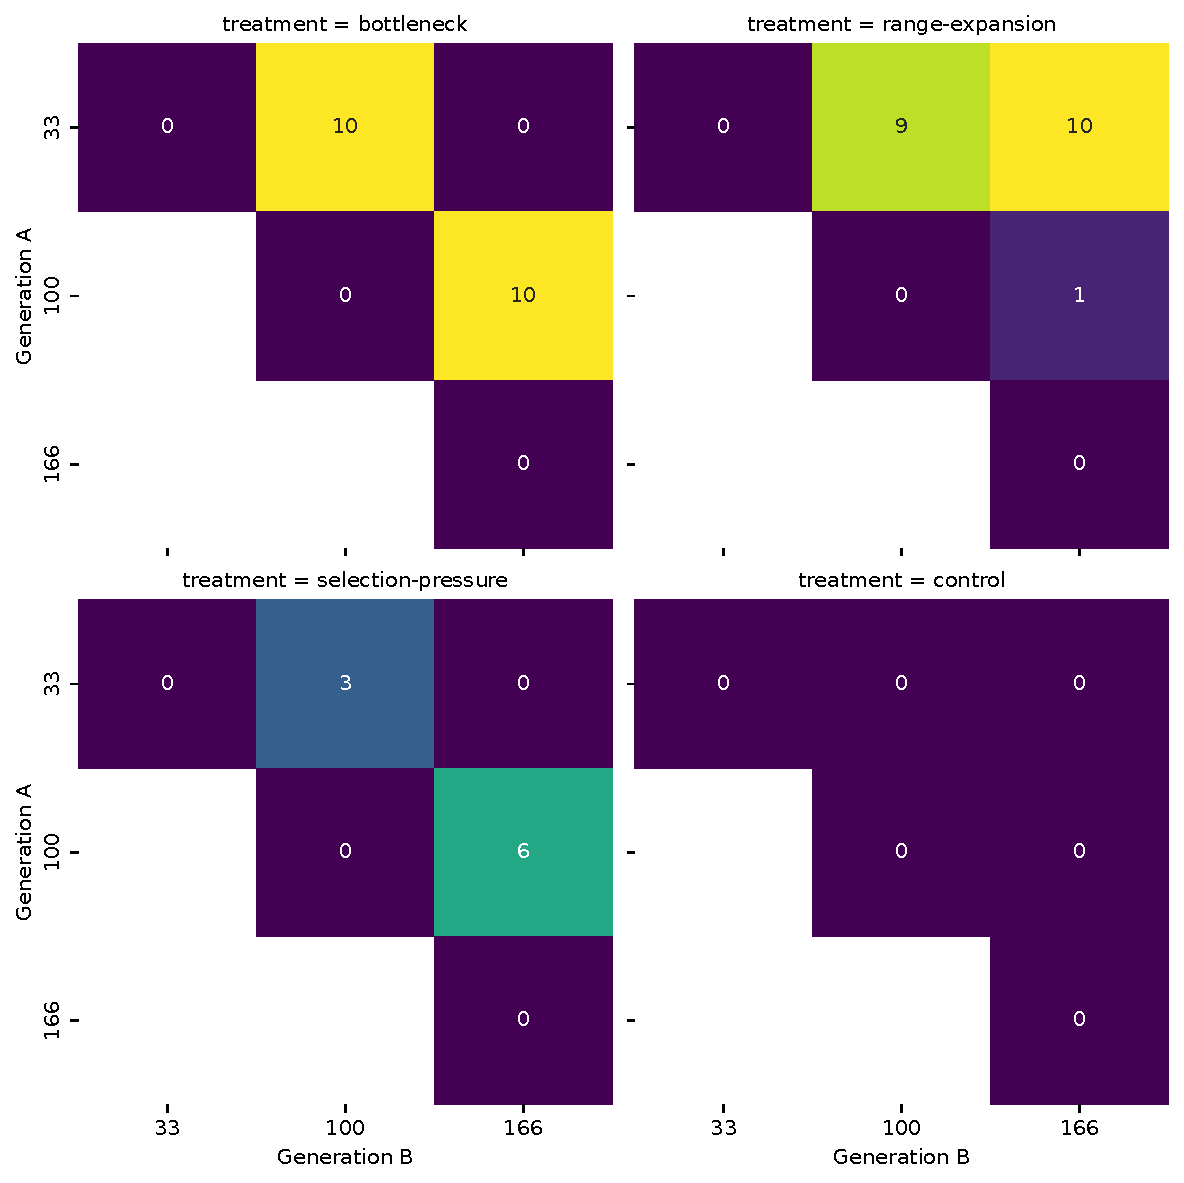
\includegraphics[width=\linewidth]{notebooks/notebooks/teeplots/hue=nonoverlapping-ci+viz=facet-heatmap+x=generation-b+y=generation-a+ext=}
    \end{minipage}%
    \begin{minipage}{0.25\textwidth}
      \caption{Non-overlapping MLE 95\% confidence intervals for rolling 10-sample estimate at target generations.}
      \label{fig:ne-detection-matrix:ci}
    \end{minipage}
  \end{subfigure}

  \caption{Counts of replicates where significant differences in effective population size ($N_e$) were detected between time point pairs.
  Counts are out of 10 total replicates attempted.
  All time point pairs had true differences in $N_e$, except same-time point pairs and time point pairs in the control experiment (Section \ref{sec:population-size-inference-experiments}.
  }
  \label{fig:ne-detection-matrix}
\end{figure}

% notebooks/notebooks/teeplots/hue=mann-whitney-significant-at-alpha-0-01+viz=facet-heatmap+x=generation-b+y=generation-a+ext=.pdf
%
% notebooks/notebooks/teeplots/hue=nonoverlapping-ci+viz=facet-heatmap+x=generation-b+y=generation-a+ext=.pdf


Figure \ref{fig:ne-detection-matrix} summarizes the detectability of underling $N_e$ changes.

Detection was performed using MLE confidnece interval comparison between rolling population size estimates at different time points and Mann-Whitney comparison of one-off population size estimate sets at different time points.

No false positives differences in effective population size are detected within the control treatment or same-timepoint comparisons within any treatment.
However, under the range expansion treatment, changes to population size from 10 to 66 is more readily detectable than changes earlier changes.

% fro mpopulation size 66 to 128.
%  \% over the course of an evolutionary run .

\subsection{Gene Selection Inference}

\begin{sidewaysfigure}
  \centering
  \vspace{0.65\textwidth}
  \begin{minipage}{.7\textwidth} % adjust the width as needed

    \begin{minipage}{\textwidth}
      \centering
      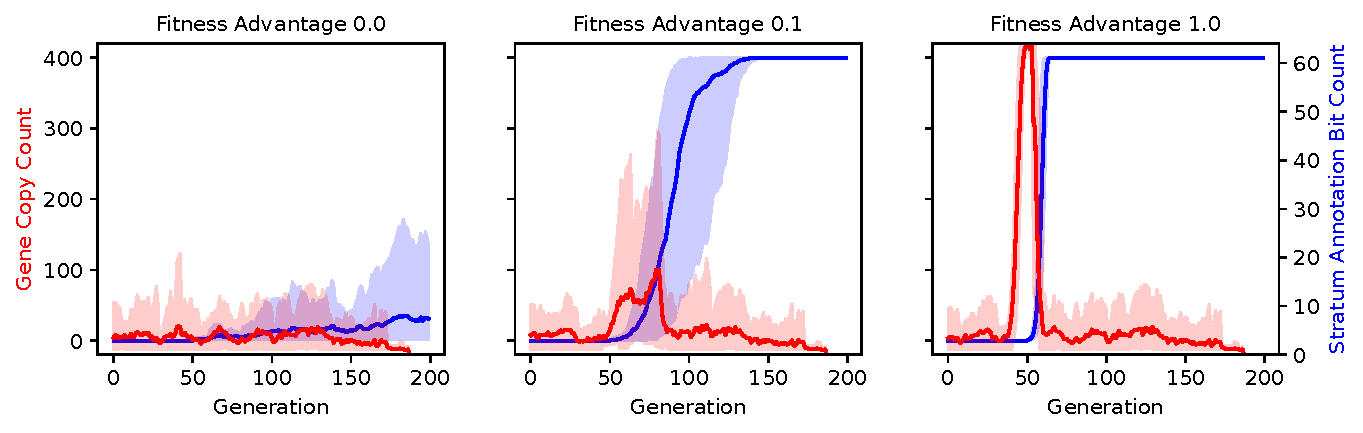
\includegraphics[width=\textwidth]{notebooks/notebooks/teeplots/col=fitness-advantage+viz=facet-lineplot-twiny+x=generation+y1=prevalence+y2=annotation+ext=}
      \subcaption{Cross-replicate aggregate, shaded bands are 95 percentile intervals}
      \label{fig:selection-example-replicates:aggregate}
    \end{minipage}

    \vspace{1cm}

    \centering
    \begin{minipage}{0.32\textwidth}
      \centering
      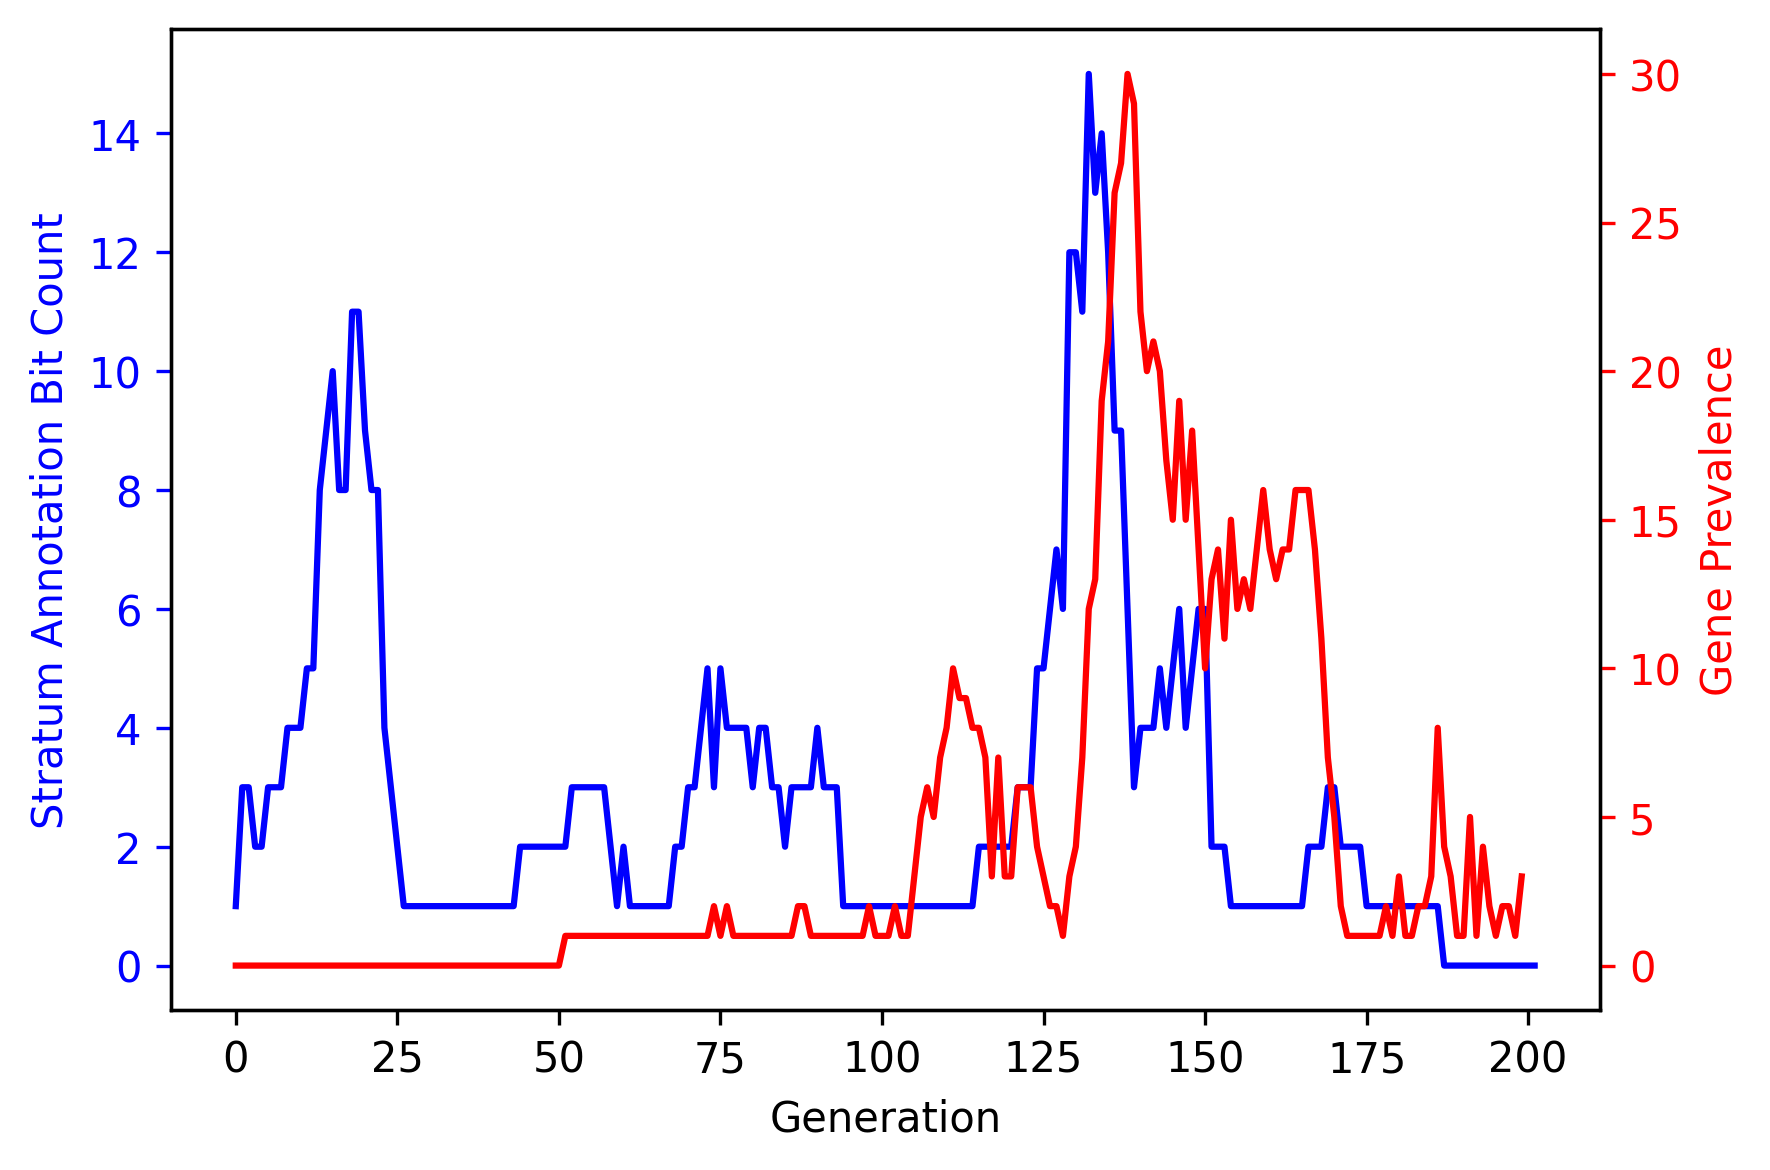
\includegraphics[width=\textwidth]{notebooks/notebooks/teeplots/fitness-advantage=0.0+notebook=gene-selection-inference+replicate=0+viz=plot-sweep-and-annotations+ext=}
      \subcaption{Example replicate with fitness advantage 0.0}
      \label{fig:selection-example-replicates:fit-0-0}
    \end{minipage}
    \begin{minipage}{0.32\textwidth}
      \centering
      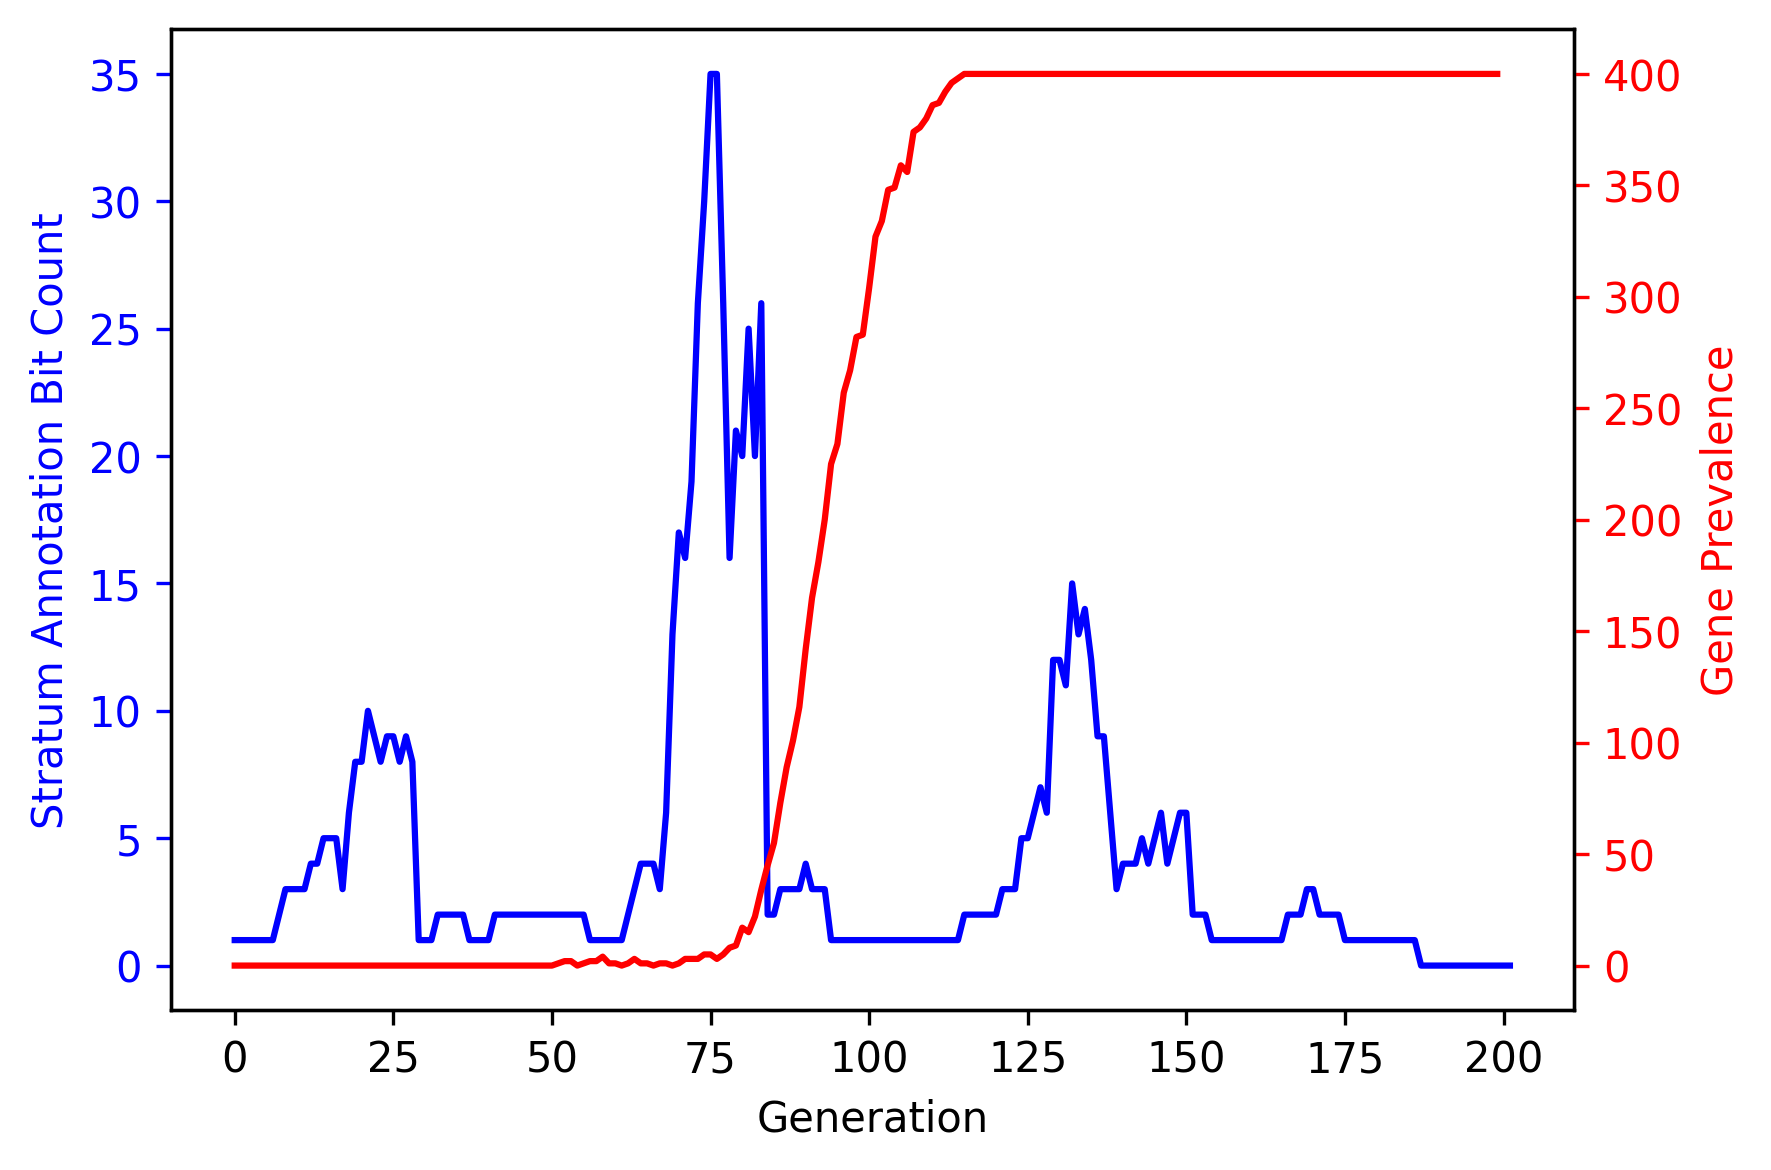
\includegraphics[width=\textwidth]{notebooks/notebooks/teeplots/fitness-advantage=0.1+notebook=gene-selection-inference+replicate=0+viz=plot-sweep-and-annotations+ext=}
      \subcaption{Example replicate with fitness advantage 0.1}
      \label{fig:selection-example-replicates:fit-0-1}
    \end{minipage}
    \begin{minipage}{0.32\textwidth}
      \centering
      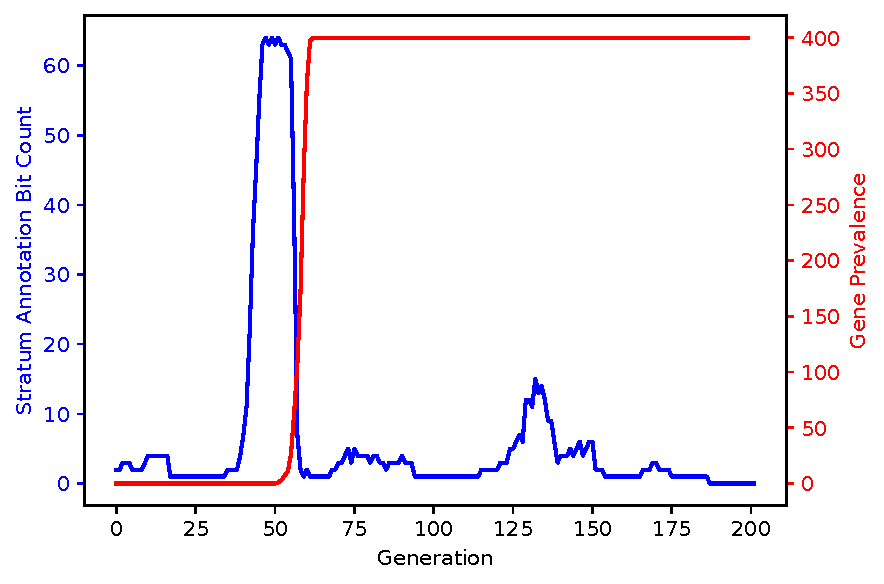
\includegraphics[width=\textwidth]{notebooks/notebooks/teeplots/fitness-advantage=1.0+notebook=gene-selection-inference+replicate=0+viz=plot-sweep-and-annotations+ext=}
      \subcaption{Example replicate with fitness advantage 1.0}
      \label{fig:selection-example-replicates:fit-1-0}
    \end{minipage}%


  \end{minipage}
  \hfill % Creates horizontal space. Can also use \hspace{<len>}
  \begin{minipage}{.25\textwidth} % adjust the width as needed
    \caption{
    Trajectories of true gene prevalence (ired) and instrument set bit counts (blue).
    Top row summarizes distribution across replicates.
    Bottom row shows an example replicate of each treatment.
    Fitness advantage 0.0 conferred no selective benefit.
    Fitness advantage 0.1 corresponded to relatively weak selection and fitness advantage 1.0 corresponded to strong selection.
    Spikes of high gene prevalence annotation bit count (blue) are used to detect underlying selective dynamics (red).
    Note that $y$ axis scaling differs among bottom-row graphs.
    }
    \label{fig:selection-example-replicates}
  \end{minipage}

\end{sidewaysfigure}


Gene selection experiments introduced novel alleles with fitness advantages of 1.0 (strong selection), 0.1 (weaker selection), and 0.0 (no selection --- control).
For each trial, the prevalence trajectory of the introduced allele and corresponding response in the distributed delayed copy count mechanism described in Section \ref{sec:positive-selection-inference-experiment} were recorded.
Copy count estimates were extracted from the hereditary stratum sequence of the focal gene's instrumentation within a randomly-sampled extant organism at the end of evolutionary runs.
The sum of copy count estimates within a sliding 16 generation window (the same duration as the copy count snapshot delay) is visualized, and was used below to detect selection events.

Figure \ref{fig:selection-example-replicates} plots these two signals for example replicates of the three treatments as well as aggregated across the ten sampled replicates.
For the strong selection treatment, allele frequency immediately shoots up towards fixation rapidly and induces a large, distinctive spike in the delayed copy count.
For the weaker selection treatment, allele frequency grows somewhat less rapidly with much greater variance in the timing of sweep culmination after allele introduction.
A delayed copy count spike is apparent, but of smaller magnitude and --- corresponding to variation in sweep culmination timing --- more variable in timing after allele introduction.
Finally, no delayed copy count spike pattern is apparent across the neutral control replicates.
However, within the visualized example control replicate run, a small magnitude spike corresponding to an apparent drift event around 150 generations can be seen.

% Gene prevalence trajectories (blue on top/red on bottom) and 16-generation rolling sums of gene prevalence annotation bit counts (red on top/blue on bottom) across generations by selection strength treatment.
% Top row summarizes distribution across replicates.
% Bottom row shows an example replicate of each treatment.
% Fitness advantage 0.0 inferred no selective benefit, so all selection detections on this treatment are false positives.
% Fitness advantage 0.1 experienced relatively weak selection and fitness advantage 1.0 experienced strong selection.
% Spikes of high gene prevalence annotation bit count (blue) are indicative of selective dynamics.
% Selection is detected for a replicate if any 16-generation rolling sum of gene prevalence annotation bit count (Section \ref{sec:dist-gene-prevalence-est}) exceeds the threshold.
% Note that $y$ axis scaling differs among bottom-row graphs.


% Gene selection detection rates across detection thresholds for each fitness advantage level among 10 replicates.
% Fitness advantage 0.0 inferred no selective benefit, so all selection detections on this treatment are false positives.
% Fitness advantage 0.1 experienced relatively weak selection and fitness advantage 1.0 experienced strong selection.
% Detection threshold 200 distinguishes treatment 0.0 and 0.1 with one false positive and one false negative.
% Fitness advantage 1.0 has all replicates detected across all shown threshold values.
% Selection is detected for a replicate if any 16-generation rolling sum of gene prevalence annotation bit count (Section \ref{sec:dist-gene-prevalence-est}) exceeds the threshold.

\begin{figure}
  \centering
  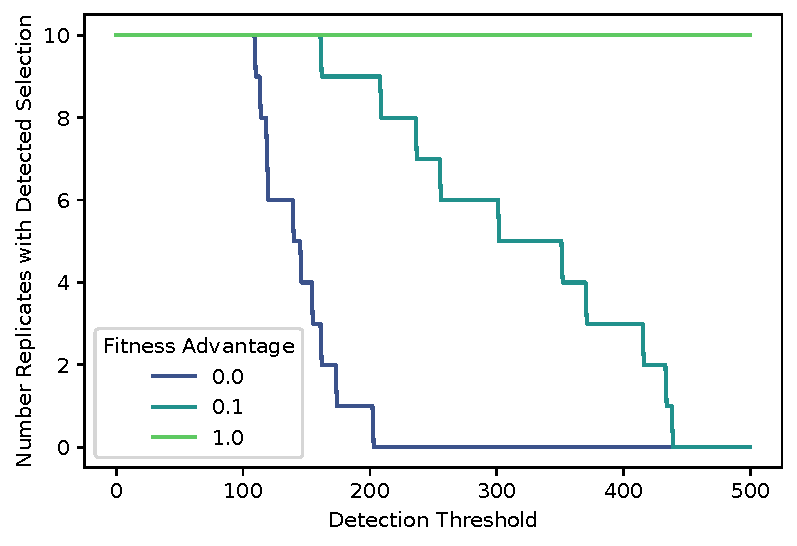
\includegraphics[width=0.8\textwidth]{notebooks/notebooks/teeplots/hue=fitness-advantage+viz=lineplot-detection+x=threshold+y=replicate-count+ext=}
  \caption{
    Gene selection detection rates by threshold for each fitness advantage level among 10 replicates.
    Fitness advantage 0.0 inferred no selective benefit, so all selection detections on this treatment are false positives.
    Detection threshold 200 distinguishes treatment 0.0 and 0.1 with one false positive and one false negative.
  }
  \label{fig:selection-sensitivity-specificity}
\end{figure}


To evaluate the sensitivity and specificity of delayed gene copy count as a mechanism for detection of selection events, we evaluated the false-positive (i.e., detection selection on control replicates) and false-negative rate (i.e., non-detection of selection on fitness-advantaged replicates) across a range of detection threshold values.
Figure \ref{fig:selection-sensitivity-specificity} plots possible trade-offs across a range of threshold values.
Strong selection events can be unambiguously distinguished from neutral events, as well as from weaker selection events.
Weaker selection and neutral events were not entirely separable.
Setting the detection threshold at sum count 200 misidentified one neutral event and one weak positive event --- corresponding to a 10\% false-positive and 10\% false-negative rate.
Better discrimination of weaker selection from neutral dynamics might be possible through longer snapshot delay, although this likely involves a trade-off with the distinctness of strong selection signal.
